%==============================================================================
% Sjabloon poster bachproef
%==============================================================================
% Gebaseerd op document class `a0poster' door Gerlinde Kettl en Matthias Weiser
% Aangepast voor gebruik aan HOGENT door Jens Buysse en Bert Van Vreckem

\documentclass[a0,portrait]{hogent-poster}

% Info over de opleiding
\course{Bachelorproef}
\studyprogramme{toegepaste informatica}
\academicyear{2023-2024}
\institution{Hogeschool Gent, Valentin Vaerwyckweg 1, 9000 Gent}

% Info over de bachelorproef
\title{Web scraping via Netwerkverkeersanalyse: Een alternatieve methode voor data-extractie}
\author{Hannes Roegiers}
\email{hannes.roegiers.student.hogent.be}
\supervisor{Sabine De Vreese}
\cosupervisor{Fabrice Luyckx (Realo)}

% Indien ingevuld, wordt deze informatie toegevoegd aan het einde van de
% abstract. Zet in commentaar als je dit niet wilt.
\specialisation{Data Engineering \& AI}
\keywords{Web scraping, netwerkverkeersanalyse, Python, Selenium}
\projectrepo{https://github.com/hannesroegiers/bachelorproef/}

\begin{document}

\maketitle

\begin{abstract}
In deze bachelorproef wordt een alternatieve methode voor webscraping geïntroduceerd en onderzocht, waarbij gebruik wordt gemaakt van netwerkverkeersanalyse. Traditionele webscraping-technieken, die vaak afhankelijk zijn van het parsen van HTML-code, stuiten op beperkingen bij het omgaan met dynamisch geladen inhoud en geavanceerde anti-scrapingmaatregelen. Dit onderzoek verkent hoe netwerkverkeersanalyse deze beperkingen kan overwinnen door data direct te onderscheppen uit het netwerkverkeer tussen de browser en de server. Het ontwikkelde Proof of Concept toont aan dat deze aanpak efficiënter is in het extraheren van gestructureerde data, vooral wanneer deze data verborgen is of dynamisch geladen wordt door de website. Daarnaast biedt de methode meer flexibiliteit en robuustheid in vergelijking met traditionele technieken. De resultaten van dit onderzoek kunnen bijdragen aan verbeterde webscraping-methoden in de toekomst, met toepassingen in diverse domeinen zoals marktonderzoek en data-analyse. Tevens worden de ethische en juridische aspecten van deze techniek besproken, waarbij de nadruk ligt op het verantwoord gebruik en de bescherming van privacy.
\end{abstract}

\begin{multicols}{2} % This is how many columns your poster will be broken into, a portrait poster is generally split into 2 columns

\section{Introductie}

In een wereld waarin data steeds belangrijker wordt als drijvende kracht achter zakelijke strategieën, wetenschappelijk onderzoek en technologische innovatie, speelt webscraping een cruciale rol. Traditionele webscraping-methoden, die voornamelijk gebaseerd zijn op het parsen van HTML-code, blijken echter vaak inefficiënt en inflexibel, vooral bij websites die hun inhoud dynamisch laden via JavaScript of andere technieken. Deze beperkingen vragen om nieuwe, innovatieve benaderingen. Dit onderzoek introduceert en verkent netwerkverkeersanalyse als een alternatieve methode voor webscraping. In plaats van te vertrouwen op de structuur van de HTML-pagina, maakt netwerkverkeersanalyse het mogelijk om data direct te extraheren uit het netwerkverkeer tussen de browser en de server, waardoor het mogelijk wordt om zelfs verborgen of dynamisch geladen data te verzamelen. Deze aanpak biedt niet alleen verbeterde efficiëntie, maar ook meer flexibiliteit, wat het een potentieel krachtige tool maakt voor data-engineers en AI-ontwikkelaars.

\section{Experimenten}

In het kader van dit onderzoek werd een Proof of Concept (PoC) ontwikkeld om de praktische toepasbaarheid van netwerkverkeersanalyse voor webscraping te testen. De experimenten richtten zich op het implementeren van een Python-script dat netwerkverkeer kan onderscheppen en analyseren om gestructureerde data te extraheren uit websites. Hierbij werden populaire Python-bibliotheken zoals Selenium, Beautiful Soup en Requests gebruikt om de kracht en beperkingen van deze techniek te onderzoeken. Een belangrijk aspect van de experimenten was het vergelijken van deze alternatieve methode met traditionele HTML-gebaseerde scraping. Het script werd getest op verschillende websites, met name die welke hun data dynamisch genereren en laden. De resultaten toonden aan dat netwerkverkeersanalyse niet alleen in staat is om data te extraheren die anders moeilijk toegankelijk zou zijn, maar ook dat het een robuuste oplossing biedt voor het omzeilen van anti-scrapingmaatregelen die vaak voorkomen bij traditionele methoden. Daarnaast werd onderzocht hoe netwerkverkeersanalyse de verwerkingstijd en de efficiëntie van data-extractie beïnvloedt, vooral in scenario's met fluctuerend netwerkverkeer.

\section{Illustratie van netwerkverkeersanalyse}

De afbeelding hiernaast toont een basisdiagram van netwerkverkeersanalyse, ook wel bekend als packet sniffing. In dit proces wordt het netwerkverkeer tussen de zender en de ontvanger onderschept en geanalyseerd door een zogenaamde "sniffer". Dit is een essentieel onderdeel van de alternatieve webscraping-methode die in dit onderzoek wordt voorgesteld. Door het verkeer tussen de browser (ontvanger) en de server (zender) te monitoren, kunnen gegevenspakketten worden onderschept die normaal gesproken niet toegankelijk zouden zijn via traditionele HTML-gebaseerde scraping. Deze aanpak stelt de onderzoeker in staat om waardevolle data te extraheren uit dynamisch geladen inhoud, wat niet alleen de efficiëntie van het scrapen verhoogt, maar ook toegang biedt tot data die anders verborgen zou blijven. Het gebruik van netwerkverkeersanalyse biedt zo een krachtige tool om nauwkeuriger en completere data te verzamelen, wat essentieel is voor data-analyse en andere toepassingen.

\begin{center}
    \captionsetup{type=figure}
    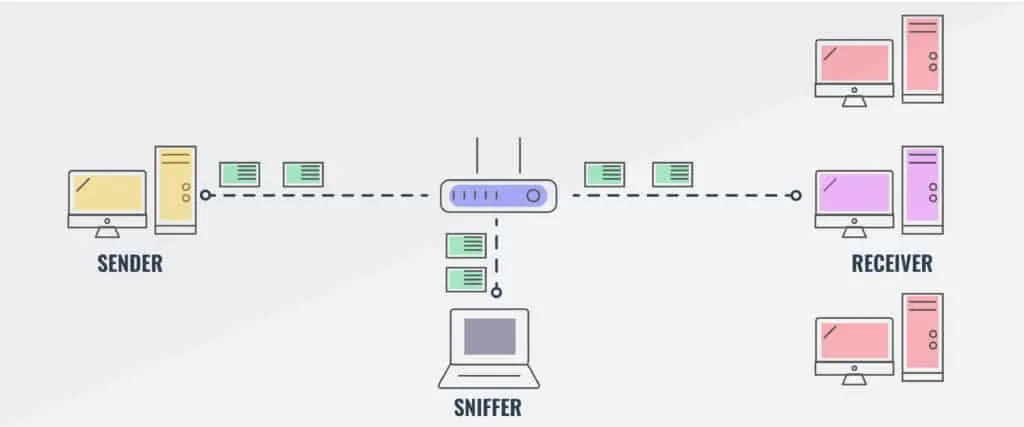
\includegraphics[width=1.0\linewidth]{graphics/networksniffing.png}
    \captionof{figure}{Een afbeelding die het onderscheppen van netwerkverkeer illustreert}
\end{center}


\section{Conclusies}

De resultaten van dit onderzoek tonen duidelijk aan dat webscraping via netwerkverkeersanalyse een krachtige en efficiënte methode is voor het extraheren van data van dynamische websites. Waar traditionele methoden vaak falen bij het omgaan met dynamisch geladen inhoud, biedt netwerkverkeersanalyse een robuust alternatief dat deze beperkingen omzeilt. Het ontwikkelde Proof of Concept illustreert hoe deze techniek niet alleen de efficiëntie van data-extractie verbetert, maar ook de flexibiliteit verhoogt door data direct uit het netwerkverkeer te halen. Dit onderzoek draagt bij aan het veld van data-engineering door een nieuw perspectief te bieden op webscraping, en biedt concrete voorbeelden en tools die kunnen worden gebruikt voor verdere ontwikkeling. De implicaties van deze resultaten zijn breed, met potentiële toepassingen in marktonderzoek, prijsvergelijking, en andere gebieden waar nauwkeurige en up-to-date data van cruciaal belang is. Bovendien benadrukken de bevindingen de noodzaak om verder te onderzoeken hoe deze methode kan worden geoptimaliseerd en toegepast in verschillende scenario's.

\section{Toekomstig onderzoek}

Hoewel de voordelen van webscraping via netwerkverkeersanalyse duidelijk zijn, opent dit onderzoek ook de deur naar verschillende vragen en uitdagingen die in de toekomst verder onderzocht moeten worden. Toekomstig onderzoek kan zich richten op het verbeteren van de efficiëntie en nauwkeurigheid van deze methode bij het omgaan met sterk beveiligde en complexe websites. Hierbij kan gedacht worden aan de ontwikkeling van technieken om versleuteld netwerkverkeer te analyseren of om te gaan met geobfusceerde data, zonder dat dit ten koste gaat van de prestaties. Daarnaast is er behoefte aan onderzoek naar de ethische en juridische aspecten van netwerkverkeersanalyse, vooral met betrekking tot privacy en gegevensbescherming. Hoe kunnen we ervoor zorgen dat deze technieken worden toegepast op een manier die in overeenstemming is met de wetgeving en ethische normen? Verder zou er ook gekeken kunnen worden naar het ontwikkelen van best practices voor het gebruik van netwerkverkeersanalyse in commerciële en academische contexten. Dit onderzoek biedt een stevige basis voor deze toekomstige inspanningen en markeert het begin van een nieuw tijdperk in data-extractie technologieën.

\end{multicols}
\end{document}